\documentclass[emulatestandardclasses]{scrartcl}
\usepackage{graphicx}
\usepackage{color}
\usepackage[ngerman]{babel}
\usepackage{hyperref}
\usepackage{fullpage}
\usepackage[dvipsnames]{xcolor}
\usepackage{calc} 
\usepackage{enumitem}
\usepackage{titlesec}
\newcommand{\todo}[1]{\textcolor{red}{TODO: #1}\PackageWarning{TODO:}{#1!}}
\date{\vspace{-3ex}}
\begin{document}

\title{
	\includegraphics*[width=0.75\textwidth]{ErstesSem/images/hu_logo.png}\\
	\vspace{24pt}
	Einf"uhrung in Kants theoretische Philosophie}
\subtitle{VEV SS 17\\
          Prof. Dr. Tobias Rosefeldt\\
          Philosophisches Institut I \\ 
          Humboldt Universit"at zu Berlin}
\author{Lennard Wolf\\
        \small{\href{mailto:lennard.wolf@student.hu-berlin.de}{lennard.wolf@student.hu-berlin.de}}}
\maketitle
\begin{abstract}

In dieser Vorlesung soll ein "Uberblick "uber die wichtigsten Themen von Kants theoretischer Philosophie gegeben werden. Im Zentrum stehen wird seine ber"uhmte These, dass alle Dinge in Raum und Zeit nur "`Erscheinungen"' sind und wir nur solche Erscheinungen, nicht aber „Dinge an sich“ erkennen können. Wir wollen untersuchen, welche philosophischen Probleme Kant zu dieser These bewogen haben, was die These eigentlich genau bedeutet und welche Rolle sie f"ur die beiden wichtigsten Aufgaben von Kants kritischer Philosophie spielt, d.h. f"ur die Erkl"arung der M"oglichkeit einer bestimmten Form apriorischen, d.h. erfahrungsunabh"angigen Wissens, und f"ur die Fundamentalkritik an den Erkenntnisanspr"uchen der traditionellen Metaphysik.

\end{abstract}
\newpage

\tableofcontents
\listoffigures
\newpage


\section{Einf"uhrung / Ausgangspunkt 1: Probleme der Metaphysik\\(20.04.17)}

\subsection{Einf"uhrung}

\subsubsection{Organisatorisches}

\begin{itemize}
  \item Selbstorganisierte Lesegruppe (optional) 
  \item Tutorientermin Do 12-14
  \item Ziel der Vorlesung: Verstehen was Kant in der KdrV haben will.
\end{itemize}

\subsubsection{Kritik der reinen Vernunft}

\begin{description}[leftmargin=!,labelwidth=\widthof{\bfseries Transzendentaler Idealismus (TI)}]
  \item[Transzendentaler Idealismus (TI)] Unterscheidung zwischen Erscheinungen und den Dingen an sich (Erstmals in der Inauguraldissertation vertreten)
  \item[Erscheinungen] Alles sinnlich wahrgenommene, Dinge die uns \emph{affizieren} und auf diese Weise uns Kenntnis von ihnen geben | Vorstellungen | Beispiele: Tische, B"aume, wir selber | Gegensatz zu Dingen an sich (auch \emph{Phaenomena}) 
  \item[Dinge an sich] Die Dinge wie sie objektiv \emph{sind}, nicht wie sie wahrgenommen werden.
  \item[Eigenschaften] Wahrgenommenes der Erscheinungen
  \item[Subjektivit"at von Raum \& Zeit] Raum und Zeit sind Bestimmungen von Erscheinungen $\rightarrow$ Dinge an sich sind nicht in Raum und Zeit sondern erscheinen uns nur so weil wir eine Anschauung in Raum und Zeit haben 
\end{description}

\subsubsection{Fragen der Vorlesung}

\begin{enumerate}
  \item {\color{NavyBlue}Was genau bedeutet die Rede von Erscheinungen und Dingen an sich?}\\
{\color{ForestGreen} Zu kl"aren.}
  \item {\color{NavyBlue} Was ist Kants philosophische Motivationslage vor 1770, die einen verstehen l"asst, weshalb er sich zu so einer extremen Position wie TI gedr"angt zu fühlen meint?}\\
{\color{ForestGreen} Zu kl"aren.}
    \item {\color{NavyBlue} Was sind Kants Gr"unde dafür TI anzunehmen?}\\
{\color{ForestGreen} Zu kl"aren.}
    \item {\color{NavyBlue} Was k"onnen wir laut Kant jeweils über Erscheinungen und
über die Dinge an sich wissen?}\\
{\color{ForestGreen} Zu kl"aren.}
    \item {\color{NavyBlue} Welche Probleme ergeben sich aus TI?}\\
{\color{ForestGreen} Zu kl"aren.}
    \item {\color{NavyBlue} Wie unterscheidet sich die Theorie der Inauguraldissertation
eigentlich von der in der Kritik der reinen Vernunft (1781), wenn doch beide TI beinhalten?}\\
{\color{ForestGreen} Zu kl"aren.}
\end{enumerate}

\subsection{Ausgangspunkt 1: Probleme der Metaphysik}

\subsubsection{Philosophische Frustration}

\begin{itemize}
  \item Problem: Philosophie besteht nur aus unkl"arbaren Streitigkeiten
  \item Kant: Das liegt daran dass es sich um metaphysische Fragen handelte und diese sind f"ur den menschlichen Verstand nicht kl"arbar
\end{itemize}


\subsubsection{Antinomien der reinen Vernunft}

\textbf{Antinomie der Teilung}

\begin{description}[leftmargin=!,labelwidth=\widthof{\bfseries Contra-Argument}]
  \item[Frage] Bestehen materielle K"orper aus einfach Teilen oder nicht?
  \item[Pro-Argument] Kompoisitionsbeziehungen bestehen immer nur kontingenterweise $\rightarrow$ Was w"are wenn alle Beziehungen aufgehoben sind? $\rightarrow$ Es m"ussen kleinste Teile existieren, denn sonst w"urde alles aus nichts bestehen
  \item[Contra-Argument] Raum besteht nicht aus Punkten und l"asst sich daher immer teilen. Damit Gegenst"ande den Raum ausf"ullen k"onnen m"ussen sie ebenso nicht punktuell sein.
\end{description}
\vspace{9pt}
\noindent \textbf{Antinomie von Freiheit und Determinismus}

\begin{description}[leftmargin=!,labelwidth=\widthof{\bfseries "Uberzeugung 2}]
  \item["Uberzeugung 1] Manchmal sind wir frei in dem, was wir tun. Wir tun
etwas, weil wir uns aus freien St"ucken dazu entschieden haben, es zu tun.
  \item["Uberzeugung 2] Alles, was in der Welt geschieht, also auch jede unserer Handlungen und Entscheidungen, ist kausal durch das determiniert, was vorher in der Welt geschehen ist.
  \item[Frage] K"onnen "Uberzeugung 1 und 2 beide wahr sein? Wenn nicht, welche ist falsch?
\end{description}


\section{Ausgangspunkt 2: Synthetische Urteile a priori\\(27.04.17)}

\subsection{Lekt"urenotizen}

\begin{itemize}
  \item Erst Erfahrung, dann Erkenntnis
  \item doch nicht alle Erkenntnis entspringt aus Erfahrung
  \item Gibt es von der Erfahrung und selbst von allen Eindrücken der Sinne unabhängiges Erkenntniß? $\rightarrow$ \emph{a priori} $\rightarrow$ Ich kann eine Erkenntnis haben ohne die daf"ur n"otige Erfahrung zu machen (Einfallen des Hauses bei Untergraben)
  \item a priori:
  \item a posteriori: empirische Erkenntnisse/ Erfahrungserkenntnisse
  \item analytisch: im Begriff selber
  \item synthetisch: \emph{irgendwie} erschlossen | WIE?
\end{itemize}

\subsection{Kants Hauptthese (Transzendentaler Idealismus)}

\begin{description}[leftmargin=!,labelwidth=\widthof{\bfseries ii}]
  \item[i] Wir m"ussen unterscheiden zwischen subjektabh"angigen Erscheinungen, d.h. den Gegenst"anden unserer sinnlichen Vorstellungen, und den Dingen, so wie sie an sich selbst beschaffen sind.
  \item[ii] Raum und Zeit sind blo"s Bestimmungen von Erscheinungen, d.h. Dinge sind nicht an sich selbst und unabh"angig von uns in Raum und Zeit.
\end{description}

\subsection{Motivation}

\begin{description}[leftmargin=!,labelwidth=\widthof{\bfseries Erkenntnistheorie}]
  \item[Metaphysik] Was zu zeigen ist: TI –- und nur TI –- kann erkl"aren, wie die widersprechenden Intuitionen zustande kommen und kompatibel gemacht werden k"onnen, und so den Streit schlichten.
  \item[Erkenntnistheorie] Was zu zeigen ist: TI –- und nur TI –- kann erkl"aren, wie diese Art von Wissen m"oglich ist. Es geht um Wissen, das in sogenannten \emph{synthetischen Urteilen a priori} zum Ausdruck kommt.
\end{description}


\subsection{Begriffe}

\begin{description}[leftmargin=!,labelwidth=\widthof{\bfseries ii}]
  \item[Was hei"st es, dass der Begriff des Unverheiratetseins in dem
des Junggesellen enthalten ist?] Alle K"orper sind ausgedehnt‘ [...] ist ein analytisch Urtheil. Denn ich darf nicht "uber den Begriff, den ich mit dem Wort K"orper verbinde, hinausgehen, um die Ausdehnung als mit demselben verkn"upft zu finden, sondern jenen Begriff nur zergliedern, d.i. des Mannigfaltigen, welches ich jederzeit in ihm denke, mir nur bewu"st werden, um dieses Pr"adicat darin anzutreffen
  \item[] 
\end{description}



%\newpage
%\section{"Uber den Professor}
%Prof. Mustermann ist..


%\begin{figure}[h]
%	\centering
%	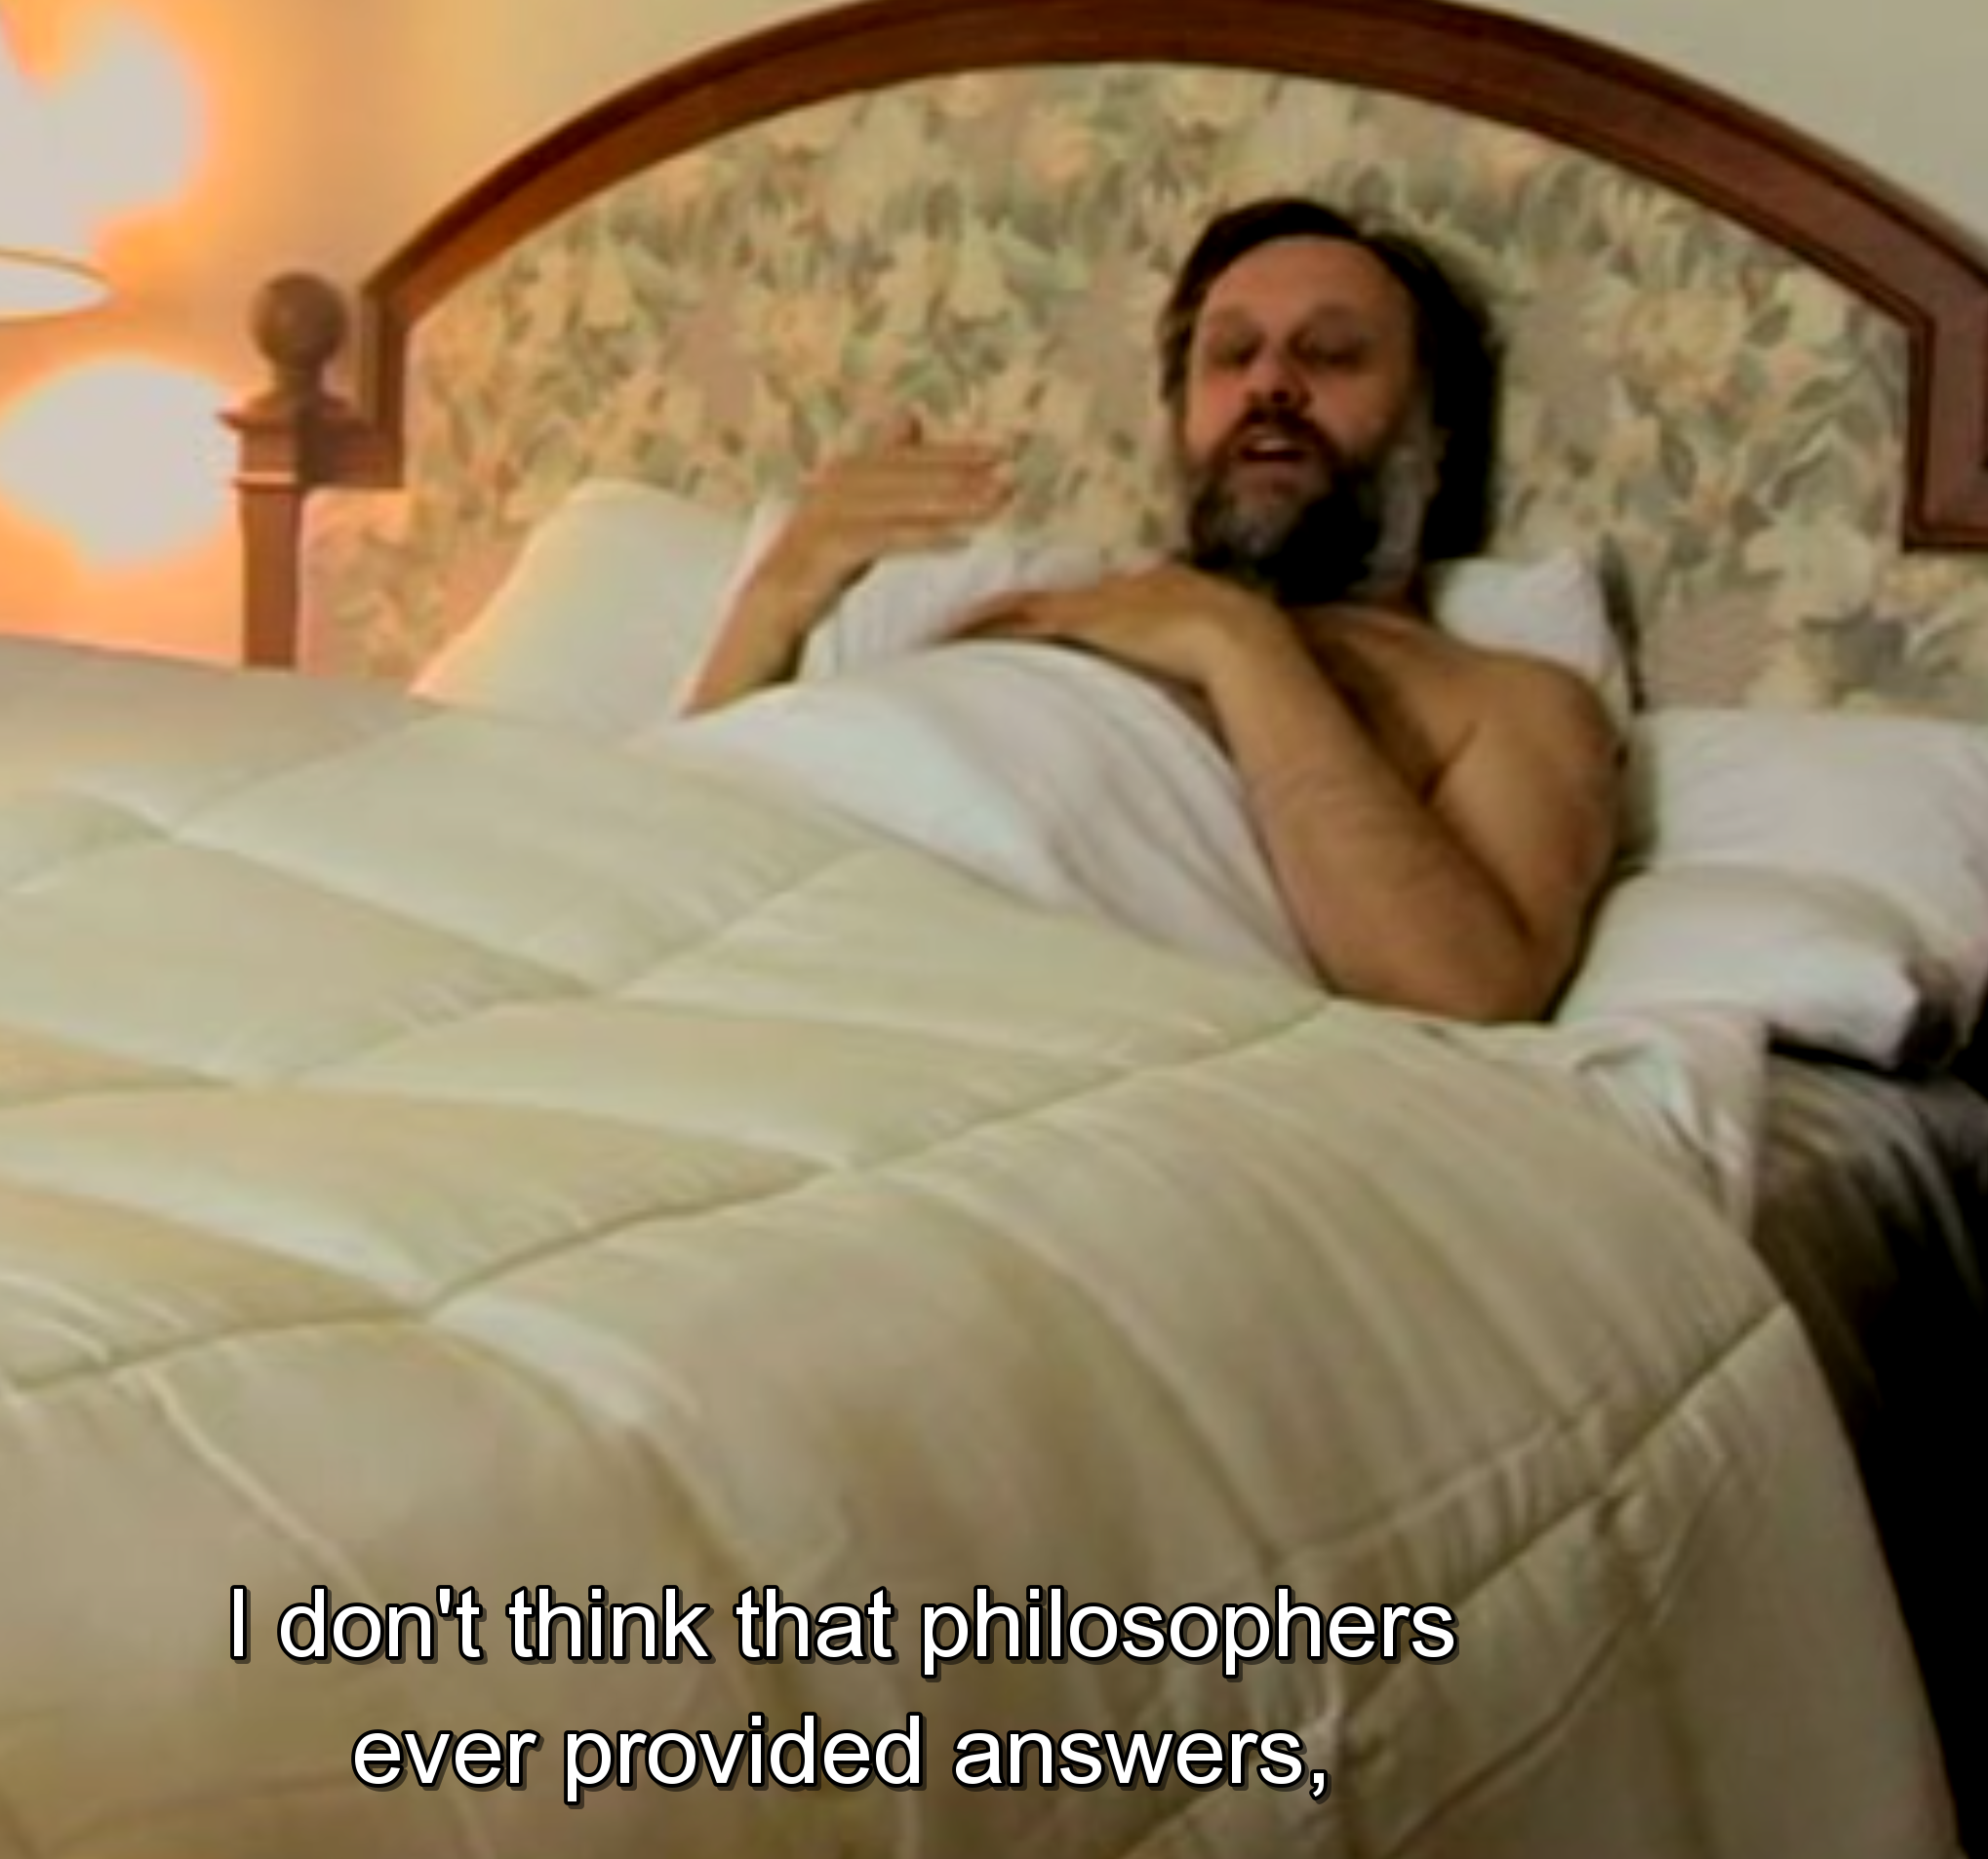
\includegraphics[width=0.5\textwidth]{images/template.png}
%	\caption{Template Bild}
%	\label{fig:template}
%\end{figure}

\end{document}


